% \usepackage{tikz}
% \usetikzlibrary{arrows}
% \usepackage{pgfplots}
% \pgfplotsset{compat=1.3}
% \usepackage[detect-family]{siunitx}
% \usepackage[eulergreek]{sansmath}
% \sisetup{text-sf=\sansmath}

\begin{sansmath}
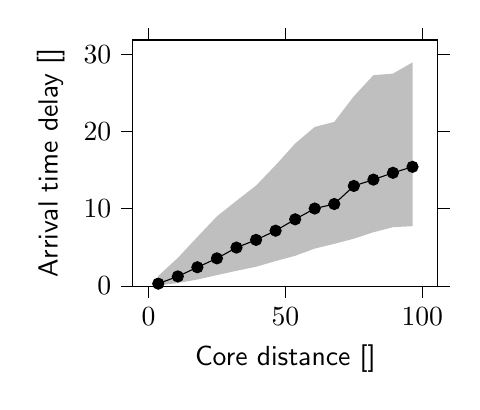
\begin{tikzpicture}[
        font=\sffamily,
        every pin/.style={inner sep=2pt, font={\sffamily\smaller}},
        every label/.style={inner sep=2pt, font={\sffamily\smaller}},
        every pin edge/.style={<-, >=stealth', shorten <=2pt},
        pin distance=2.5ex,
    ]
    \begin{axis}[
            width=.45\linewidth,
            %
            xlabel={ Core distance [\si{\meter}] },
            ylabel={ Arrival time delay [\si{\nano\second}] },
            %
            xmin={  },
            xmax={  },
            ymin={ 0 },
            ymax={  },
            %
            xtick={  },
            ytick={  },
            %
            tick align=outside,
            max space between ticks=40,
            every tick/.style={},
        ]

        
            \addplot[draw=none, fill=lightgray] coordinates {
                (3.57142857143, 0.0698878)
                (10.7142857143, 0.401903741062)
                (17.8571428571, 0.845024)
                (25.0, 1.4196164608)
                (32.1428571429, 1.9764)
                (39.2857142857, 2.50102418661)
                (46.4285714286, 3.23459517956)
                (53.5714285714, 3.92207)
                (60.7142857143, 4.85639941692)
                (67.8571428571, 5.47321)
                (75.0, 6.13938069344)
                (82.1428571429, 6.97056281567)
                (89.2857142857, 7.62987554073)
                (96.4285714286, 7.75882923603)
                (96.4285714286, 28.9807648659)
                (89.2857142857, 27.5304198265)
                (82.1428571429, 27.3245458603)
                (75.0, 24.5882492065)
                (67.8571428571, 21.2758)
                (60.7142857143, 20.6196737289)
                (53.5714285714, 18.4657)
                (46.4285714286, 15.6637165546)
                (39.2857142857, 13.0215501785)
                (32.1428571429, 11.0533)
                (25.0, 9.0351524353)
                (17.8571428571, 6.36103)
                (10.7142857143, 3.65638321638)
                (3.57142857143, 1.31555)
                } -- cycle;
        

        
            \addplot[mark=*,solid] coordinates {
                (3.57142857143, 0.313231)
                (10.7142857143, 1.25172072649)
                (17.8571428571, 2.4365)
                (25.0, 3.58899)
                (32.1428571429, 4.98443)
                (39.2857142857, 5.98225998878)
                (46.4285714286, 7.17367267609)
                (53.5714285714, 8.64839)
                (60.7142857143, 10.0465011597)
                (67.8571428571, 10.6293)
                (75.0, 12.9728)
                (82.1428571429, 13.7917895317)
                (89.2857142857, 14.6759257317)
                (96.4285714286, 15.4506721497)
            };
        

        
    \end{axis}
\end{tikzpicture}
\end{sansmath}